%https://www.overleaf.com/project/5eceb90a9c86e30001cec720

\documentclass[12pt]{revtex4}
%\usepackage[demo]{graphicx}% Include figure files
\usepackage{dcolumn}% Align table columns on decimal point
\usepackage{bm}% bold math
\usepackage[utf8]{inputenc}
\usepackage{graphicx}
%\graphicspath{ {./images/} }



\voffset 1.0cm

\begin{document}
\linespread{1.5}
\title{ Detection of COVID-19 Using Chest X-ray Images by Convolutional Neural Networks}
\author{Aanchal Dusija \\ Meghnad Desai Academy of Economics}
\date{July 18, 2020}

%how to add page number in bottom centre?
%how to shift abstract more down?
\begin{abstract}
The outbreak of COVID-19 has caused distress and chaos in the entire world with the exponential growth of cases. Priority calls for social distancing and quarantine, the only ways of preventing the spread of the disease. It has been observed that the RT-PCR testing of COVID-19 is not only resulting in many false results but is also time-consuming. Therefore, immediate and efficient testing of COVID-19 is essential with the widespread disease over all the continents. Alternative detection techniques are the need of the hour to combat the disease. In this paper, an automated detection system is built to detect COVID-19 using Chest X-rays Images with the aid of Convolutional Neural Network (CNN). The CNN model has given the accuracy of 97\% in the detection of COVID-19 and Normal Chest X-ray Images. 
\\Keywords: COVID-19, RT-PCR, Chest X-rays, Convolutional Neural Network. 
\end{abstract}

\maketitle

\pagebreak
\section{Introduction}
The recent outbreak of a transmissible disease known as COVID-19 has caused a global alarm. COVID-19 is an infectious disease caused by a recently discovered coronavirus. The outbreak commenced in December 2019 in the city of Wuhan, China which soon turned into a pandemic due to its contagious nature. It is also called as Severe Acute Respiratory Syndrome Coronavirus 2 (SARS-CoV-2). [web1]
\\Coronaviruses (CoV) are a family of hundreds of viruses that usually infect animals like chickens, bats, camels, cats. These viruses within the animals can mutate permitting them to transmit the virus within them to other species leading to a spill-over [web2]. It has been observed that the virus is mainly attacking the respiratory system in humans, ranging from the common cold to more deadly diseases like Middle East Respiratory Syndrome (MERS) and Severe Acute Respiratory Syndrome (SARS).
\\The symptoms of COVID-19 can be very mild; some people may not show any symptoms at all but can infect other people. It is not as deadly as SARS and MERS [paper1]. The most common symptoms of COVID-19 are fever, dry cough, and fatigue. Other symptoms that are less common in nature are headaches, nasal congestion, sore throat, loss of taste and smell, conjunctivitis, and discolouration of fingers or toes. Usually, older people having other underlying medical problems like high blood pressure, heart and lung problems, diabetes, or cancer are at a higher risk of developing a severe illness. However, anyone can get the virus and get seriously ill.
\\In many developed countries, the health system has come to the point of collapse due to the increasing demand for intensive care units simultaneously [paper2]. Intensive care units are filled with patients who get worse with COVID-19 pneumonia. Coronavirus is continuing its spread across the world, with more than 11 million confirmed cases in 188 countries. At least half a million people have lost their lives, as per 7th July, 2020 [web5]. 
%(CNN_WORLD)
\begin{figure}[htp]
    \centering
    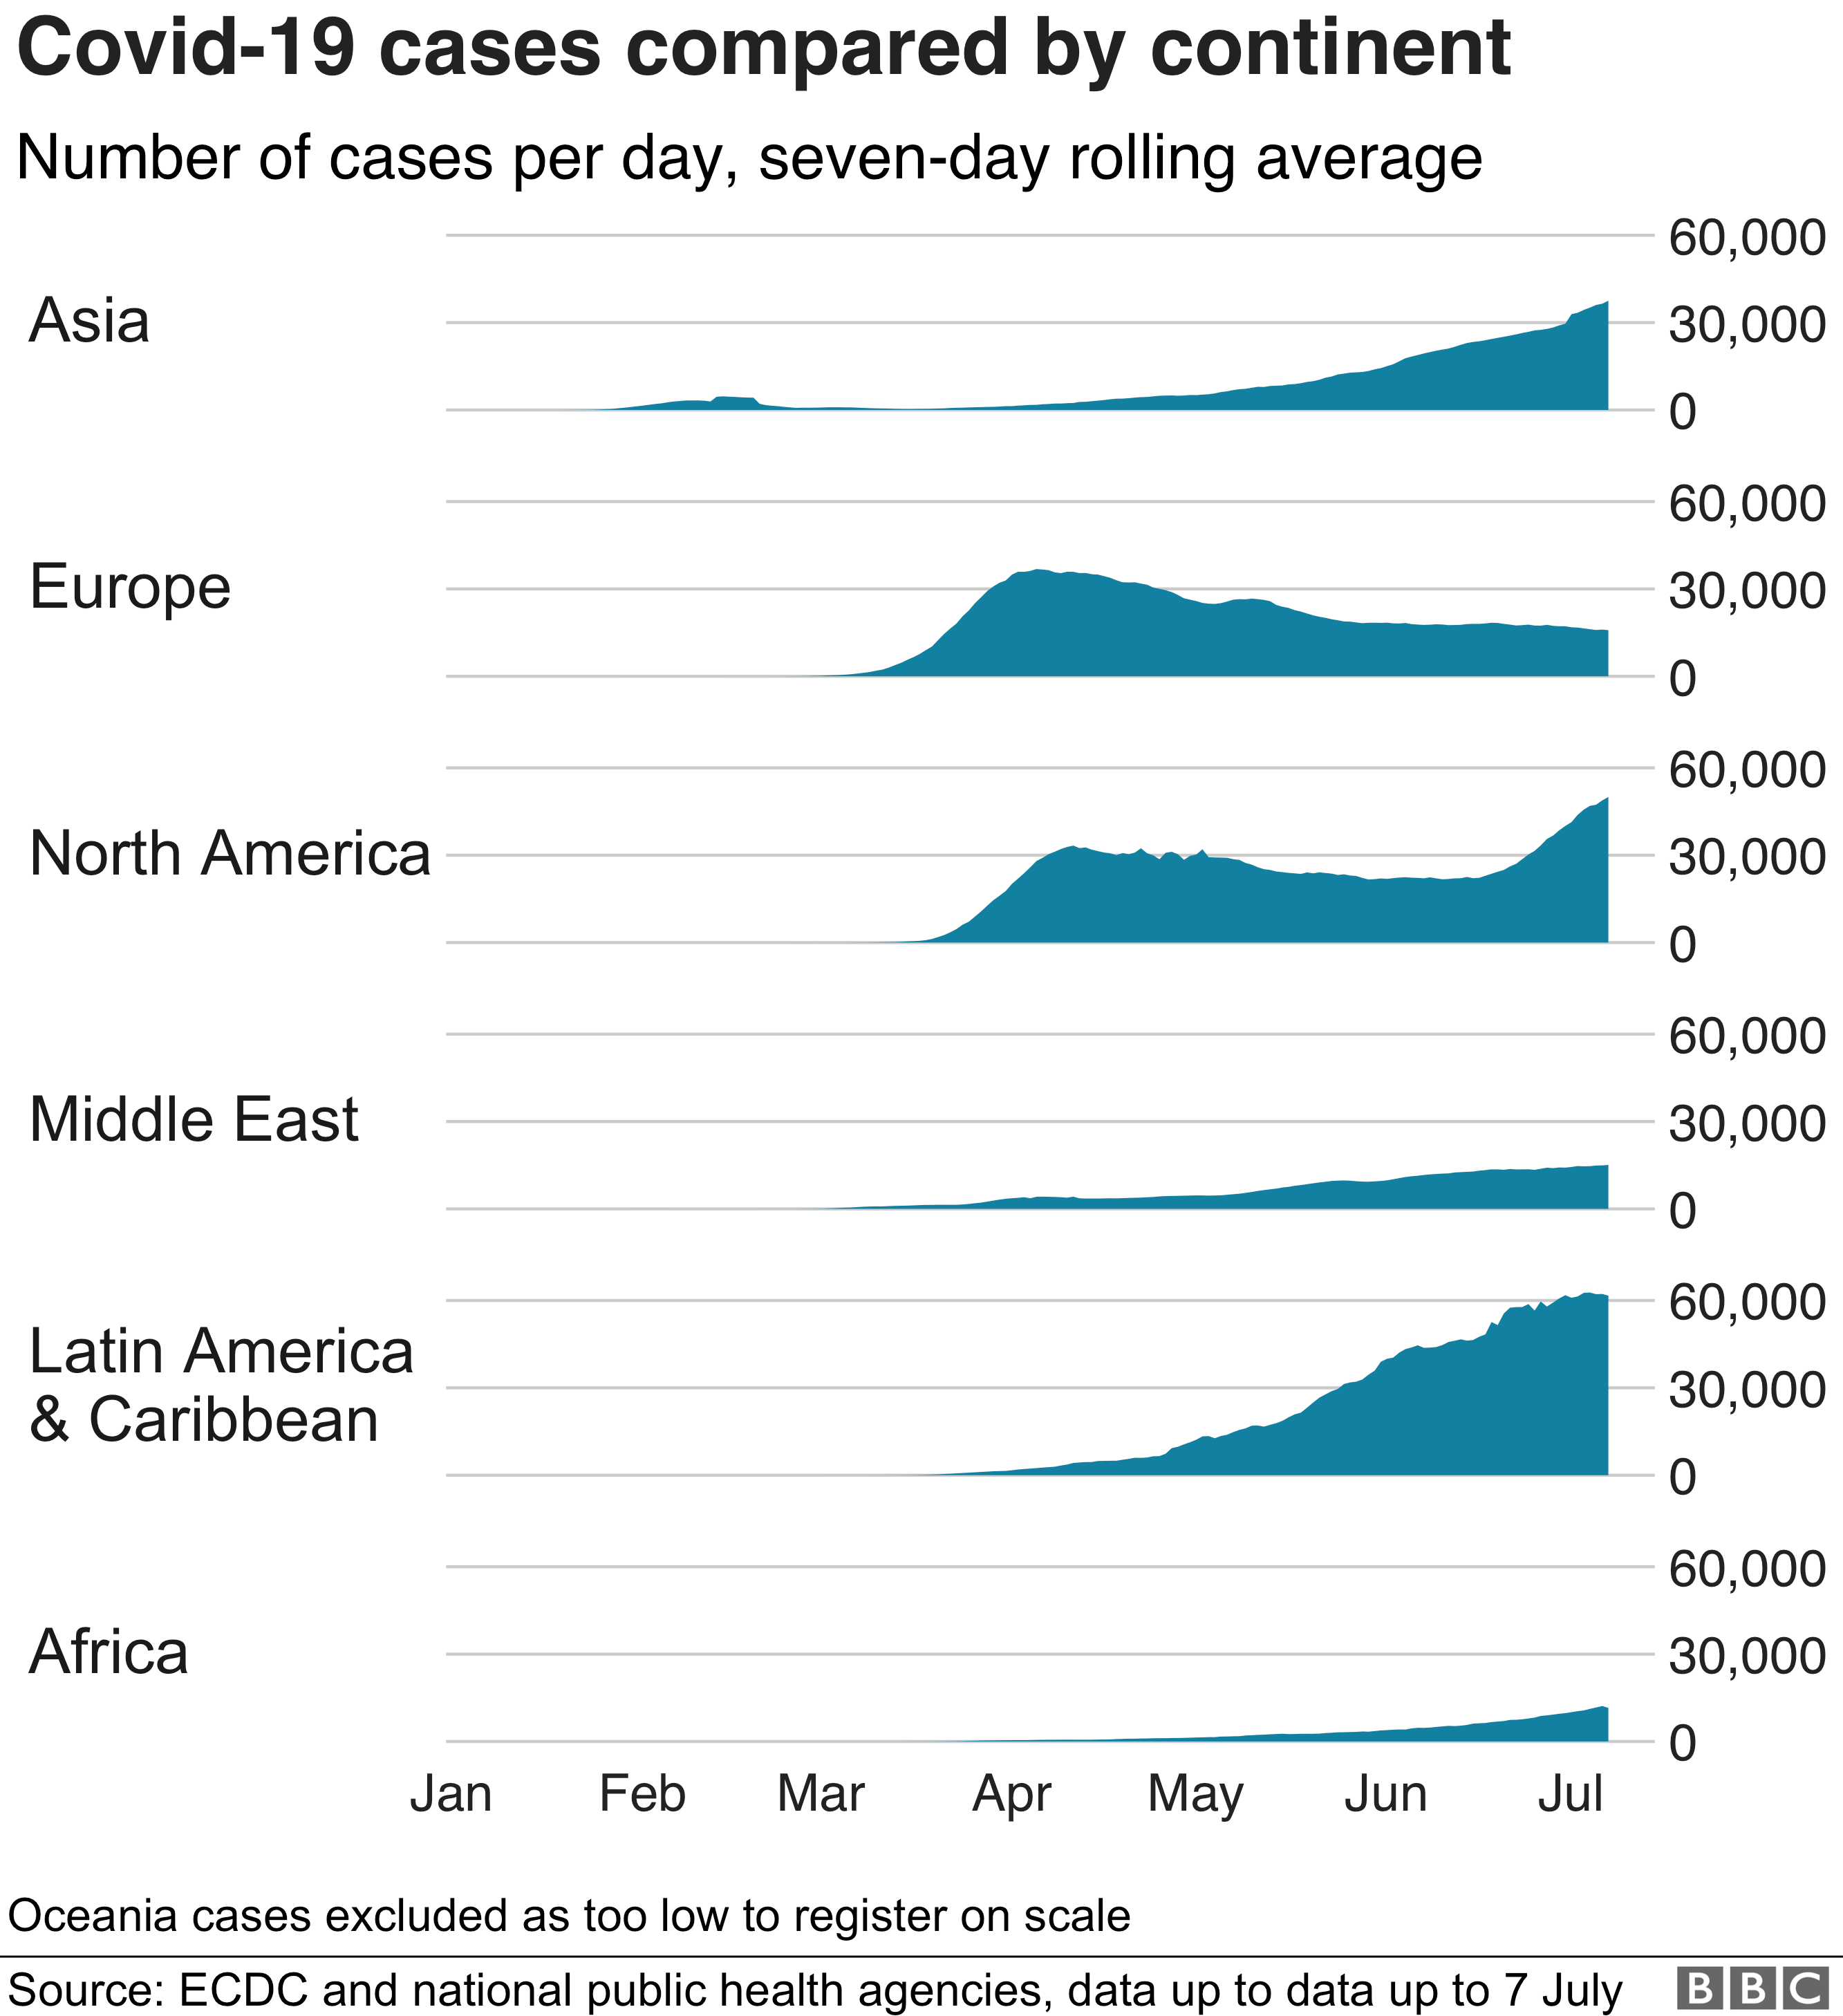
\includegraphics[width=16cm]{CNN_World.png}
    \caption{Spread of COVID-19 over the Continents}
    \label{fig:def}
\end{figure}
\\The disease has spread across the globe in the first few months of 2020, reaching 10 million cases. Europe and North America saw the first major outbreaks in April but as they began to ease, Latin America and Asia started seeing an increase in cases. North America has seen a resurgence of infections in recent weeks, mostly driven by new outbreaks in the US, but Mexico has also seen an increasing number of cases.
\\Not only this, COVID-19 has brought economic activity in the entire world at a standstill. The economic damage is evident. This pandemic is one of the largest economic shock the world has experienced in decades. Recent data shows that the service industry has been hit the hardest. Tourism and global trade have been massively disrupted in every region of the world. The World Trade Organization (WTO) expects global trade to fall up to 32\% this year due to the coronavirus pandemic [paper5]. The deep recession triggered by the pandemic are expected to leave ever lasting scars through lower investment, an erosion of human capital and fragmentation of global trade and supply linkages. 
\\SARS, which was first detected in November 2002, bears several similarities to COVID-19. Both the coronaviruses are believed to have originated from bats, jumping to humans via an intermediate animal host [web2]. According to the WHO, SARS punched holes in the lungs, giving them “a honeycomb-like appearance” [paper2] —and these lesions are present in those afflicted by a novel coronavirus, too. However, the mortality rates for SARS are higher. In 2012, there was another outbreak of a newly found coronavirus called the Middle East Respiratory Syndrome (MERS). The very first case was found in Saudi Arabia. The difference between SARS, MERS, and COVID-19 is that R0 for SARS is 3, R0 for MERS is less than one, but the R0 for COVID-19 is 5, meaning that every infected person is likely to infect five other people. This shows how the infectious nature of COVID-19 [web2].
\\COVID-19 begins and ends in patients’ lungs, because like the flu, coronaviruses are respiratory diseases. They spread typically when an infected person coughs or sneezes, spraying droplets that can transmit the virus to anyone in close contact. Coronaviruses also cause flu-like symptoms: Patients might start with a fever and cough that progresses to pneumonia or worse [web3].
\\COVID-19 is detected in the upper and lower respiratory specimens of the individuals with the help of RT-PCR (real-time transcription-polymerase chain reaction) test. Since the origin of the outbreak, the availability and quantity of the testing kits have been low. The stability and reproducibility if the detection kits are being questioned. These factors play a determinant role in the accuracy of test results. In several areas, the accuracy of the kits has found to be only 80\% and has to be hence repeated several times before the cases can be confirmed. There are questions being raised about quality and stability of the detection kits [web4].
\\X-ray images of the chest can be used to diagnose COVID-19 with technological advancements made in the field of machine learning. One of the most vital methods of machine learning is deep learning. Deep learning focuses on extracting features and classifies images which are applied in detecting objects or in medical cases, classification of tasks. Machine learning and deep learning have become established disciplines in applying artificial intelligence to mine, analyze, and recognize patterns from data [paper3]. 
\\With the recent innovation in Artificial Intelligence (AI), COVID-19 can be detected, quantified, and monitored and making it easier to isolate patients who have been infected for faster treatment. Chest x-rays scan the infections present in the lungs of the patient. It is a faster, easier, cheaper, and less harmful method of testing patients and hence must be used. With the increasing mortality rates all thanks to COVID-19, Chest X-rays must be implemented by all countries on an urgent basis. Although this technological advancement seems helpful, the images of various types of pneumonia are similar and overlap with other infectious and inflammatory lung diseases making it difficult to distinguish between COVID-19 from other viral cases of pneumonia [paper2].
\\In the study, a prediction of the COVID-19 detector will be modelled using Convolutional Neural Network (CNN) based on Chest x-rays images. CNN helps in the extraction of the features by enhancing low-light images with the help of training data. In the early stages of COVID-19, bilateral distribution of patchy shadows and ground-glass opacity has been observed which are similar to the viral pneumonia symptoms with slight differences [paper1]. With the aid of the CNN model, unique features can be identified which are difficult for visual recognition. After the model is trained on the dataset, performance of this classification model is evaluated on the validation dataset using a Confusion Matrix. 
\pagebreak
\section{Literature Review}
Convolutional neural network (CNN) is one of the most popular and effective approaches in the diagnosis of COVD-19 from digitised images. Several reviews have been carried out to highlight recent contributions to COVID-19 detection.
\\In Shuai et al. study, based on the COVID-19 radiographic changes from CT images, they have developed a deep learning method that can extract the graphical features of COVID-19 to provide clinical diagnosis prior to pathogenic testing and thus save critical time for the disease diagnosis [paper1].
\\In a study by Apostolopoulos et al., a dataset of X-ray images from patients with pneumonia, confirmed Covid-19 disease, and normal incidents, was used to evaluate the performance of state-of-the-art convolutional neural network architectures proposed previously for medical image classification. The study suggested that transfer learning can extract significant biomarkers related to the Covid-19 disease [paper4].
\\In a study by Narin et al., pre-trained models like ResNet50, InceptionV3 and Inception-ResNetV2 are used on a chest x-ray dataset to distinguish between COVID-19 and normal images [paper2]. 
\\In a study by Abbas et all., a detection system has been made using the DeTraC deep convolutional neural network to classify images of Normal, COVID-19 and SARS chest x-ray images [paper6].
\\In a study by Basu et al., a detection system has been built to differentiate between CPVID-19 and Pneumonia chest x-ray images using Domain Extension Transfer Learning and Thoracic Imaging. They have also detected the regions in which the infection has spread in the chest x-rays using Gradient Class Activation Map (Grad-CAM) [paper7]. 
\\In a study by Fei et al., they developed a deep learning-based system for automatic segmentation of all lung and infection sites using chest CT [paper9]. 
\\Xiaowei et al. aimed to establish an early screening model to distinguish COVID-19 pneumonia and Influenza-A viral pneumonia from healthy cases using pulmonary CT images and deep learning techniques [paper8]. 


\pagebreak
\section{ Math Behind CNN}
Convolutional Neural Network (CNN) is a robust deep learning algorithm, mainly used to identify and classify images. CNN is a distinctive type of neural network in which analyses visual inputs to identify for segmentation, detection, and classification. The concept is based on combining low-level features in the image to higher and higher-level features. The filters extract features from images in such a way that the position information of pixels is retained. The algorithm is mainly used for face recognition, analysing documents, managing traffic in smart cities, and recommendation systems.
\\CNN is trained on the back-propagation algorithm. After we get the output from Forward propagation, the actual value is compared with the output to calculate the error rate. The parameters are then updated, and the entire process is repeated to get the optimal values. [1]
% (https://www.analyticsvidhya.com/blog/2020/02/mathematics-behind-convolutional-neural-network/?utm_source=blog&utm_source=learn-image-classification-cnn-convolutional-neural-networks-5-datasets)
 \\CNN is an amalgamation of biology, art, and mathematics. The biology of the eye inspires the entire architecture. CNN mimics the connectivity of neurons within the brain. While we as humans perceive a visual image as a detailed, coloured image of the world around us, there is quite a lot of processing done in our brain to get to this point. 
\\CNN has proved particularly successful in working with image data and ever since being used in ImageNet competition in 2012. They have been the frontrunners in research and industry while dealing with images.[2]
%https://courses.analyticsvidhya.com/courses/convolutional-neural-networks-cnn-from-scratch?utm_source=blog&utm_medium=mathematics-behind-convolutional-neural-network
\\CNN can also be used for deep learning applications in healthcare, such as medical imaging. CNN has been used for features learning on breast ultrasound images, blood analysis, brain lesion segmentation, detection of Alzheimer’s and Parkinson’s Diseases, tumour, lung cancer, pneumonia, and various other diseases. [3] 
%(https://arxiv.org/ftp/arxiv/papers/1704/1704.06825.pdf) 
\\The neurons within a CNN are split into a three-dimensional structure, with each set of neurons analysing a small region or feature of the image. In other words, each group of neurons specializes in identifying one part of the image. CNNs use the predictions from the layers to produce a final output that presents a vector of probability scores to represent the likelihood that a specific feature belongs to a certain class. [4]
%https://missinglink.ai/guides/convolutional-neural-networks/convolutional-neural-network-architecture-forging-pathways-future/
\\CNN is composed of several kinds of layers:
\\\textbf{1) Convolutional Layer:}
\\This layer3 consist of Image Filters that extract patterns from the image. What information these filters extract is learned, just like in the brain. When we train a Convolutional Neural Layer, we try to generate the best possible filters, e.g. the filters that extract the most meaningful information. 
\\Convolutional layers detect low-level features such as edges and curves. This layer creates a feature map to predict the class probabilities for each feature by applying a filter that scans the whole image, a few pixels at a time.

%Image has to be inputted
\begin{figure}[htp]
    \centering
    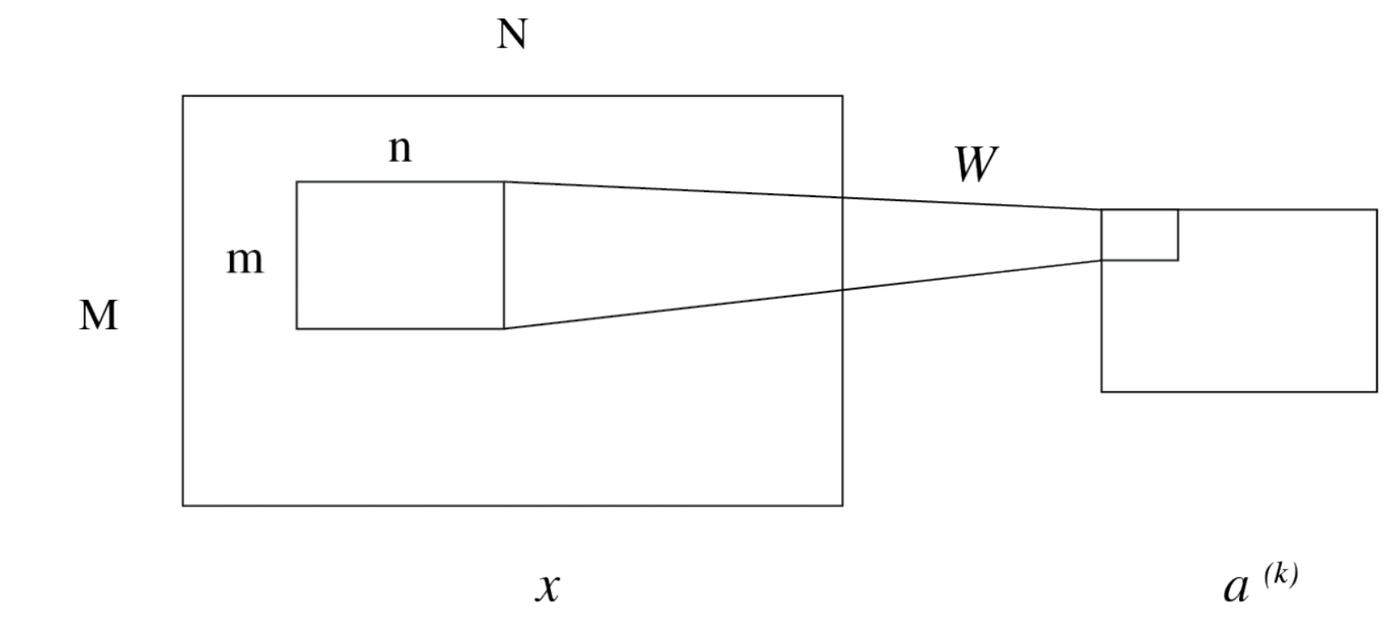
\includegraphics[width=16cm]{CNN_Math.png}
    \caption{Convolutional Layer}
    \label{fig:abc}
\end{figure}
Let's consider a single image case. For simplicity, I would like to define the image size and its convoluted image
size as above.
\\So notation here is like below.
\\$x$: input
\\$a^{k}$: after convoluted image
\\$k$: index of kernel (weight filter)
\\$W$ : kernel (weight filter)
\\$b$: bias
\\$E$: cost function
\\CNN follows the forward propagation procedure in which the weights, biases and filters are inputted, processed and passed on to its successive layers. These values act as parameters of the CNN model. 
\begin{equation}a_{i j}^{(k)}=\sum_{s=0}^{m-1} \sum_{t=0}^{n-1} W_{s t}^{(k)} x_{(i+s)(j+t)}+b^{(k)}\end{equation}
\\The activation function is the non-linear transformation that we do over the input signal. This transformed output is then advanced to the next layer of neurons as input. When it comes to the selection of activation functions, indeed we have some options, for example, ReLU, sigmoid or hyperbolic tangent. They are given as follows: 
\\Sigmoid Function: $\frac{1}{1+e^{-x}}$
\\tanh Function: $tanh (x)$
\\ReLU Function: $max (0, x)$
\\Leaky ReLU Fucntion: $max(0.1x,x)$
\\Maxout Function: $\max \left(w_{1}^{T} x+b_{1}, w_{2}^{T} x+b_{2}\right)$
\\ELU Function: $\left\{\begin{array}{ll}
x & x \geq 0 \\
\alpha\left(e^{x}-1\right) & x<0
\end{array}\right.$
\\ReLU function is the most widely used activation function in neural networks. ReLU converts all negative inputs to zero, and the neuron does not get activated, making it very computational efficient as few neurons are activated per time. It does not saturate at the positive region. The ReLU activation functions is used for the hidden layers.
\begin{equation}a_{i j}=\max \left(0, x_{i j}\right)\end{equation}
\\\textbf{2) Pooling Layer(Down-Sampling:}
\\Even though the size of the images will slightly decrease with each filter in each layer, we generally generate exponentially more and more data with each convolutional layer we add. To combat this issue, we use a process called Pooling. In this layer, the amount of information generated by the convolutional layer is scaled-down and only saves crucial information. Most prominently, we use Max Pooling, meaning we take the maximum pixel value of a pixel neighbourhood.
\begin{equation}a_{i j}=\max \left(0, x_{(i+s)(j+t)}\right)\end{equation}
where $s \in|0, l|$ and $t \in|0, l|$ and $l$ is filter size.
\\\textbf{3) Fully Connected Layer:}
\\This layer “flattens” the outputs generated by previous layers to turn them into a single vector that can be used as an input for the next layer. It converts a two-dimensional convolutional layer into one dimension which can be used to connect to the fully connected layer.  The weights are applied over the input generated by the feature analysis to predict an accurate label.
\\\textbf{4) Fully Connected Output Layer:}
\\A fully connected layer uses the output of the convolution layer to predict the best description for the image. This layer generates the final probabilities to determine a class for the image. Sigmoid function is a S-Shaped curve which is differentiable and monotonic in nature, existing between 0 and 1. The sigmoid activation function is used for the output layer because there is a distinction to be made between two classes. 
\begin{equation}a_{i j}=\frac{1}{1+e^{-x}}\end{equation}
\\A technique called forward-backward propagation is used to check and optimize the performance of the model. In forward propagation, the input data is fed in the network, and the output data is generated. The loss is calculated to see how far away the prediction of the network is from the actual value. We calculate the cross-entropy error of the model: 
\begin{equation}crossentropy=-(1 / n)\left(\sum_{i=1}^{n}\left(y_{i} \times \log \left(O_{\text {outi}}\right)\right)+\left(\left(1-y_{i}\right) \times \log \left(\left(1-O_{\text {outi}}\right)\right)\right)\right)\end{equation}
\\In the backward propagation process, the parameters of the model are updated in a manner that the overall predictions are more accurate than the previous model. This composition has to be optimized on a per-layer basis. The error can be propagated back from the end to the start by de-stacking through the function calls. This technique is called auto-differentiation and requires only that each function is provided with the implementation of its derivative.
\\Back propagation of the Convolutional layer:
\\i) Back propagation to Update the Weights:
\begin{equation}\begin{array}{c}
\frac{\partial E}{\partial W_{a t}^{(k)}}=\sum_{i=0}^{M-m} \sum_{j=0}^{N-n} \frac{\partial E}{\partial a_{i j}^{(k)}} \frac{\partial a_{i j}^{(k)}}{\partial W_{n t}^{(k)}}=\sum_{i=0}^{M-m} \sum_{j=0}^{N-n} \frac{\partial E}{\partial a_{i j}^{(k)}} x_{(i+a)(t+t)} \\
\frac{\partial E}{\partial b^{(k)}}=\sum_{i=0}^{M-m} \sum_{j=0}^{N-n} \frac{\partial E}{\partial a_{i j}^{(k)}} \frac{\partial a_{i j}^{(k)}}{\partial b^{(k)}}=\sum_{i=0}^{M-m} \sum_{j=0}^{N-n} \frac{\partial E}{\partial a_{i j}^{(k)}}
\end{array}\end{equation}
Bear in mind that the propagated error can be noted like below.
\[
\delta_{i j}^{k}=\frac{\partial E}{\partial a_{i j}^{(k)}}
\]
\\ii) Back propagation to Previous Layer:
\begin{equation}\frac{\partial E}{\partial x_{i j}}=\sum_{s=0}^{m-1} \sum_{t=0}^{n-1} \frac{\partial E}{\partial a_{(i-s)(j-t)}^{(k)}} \frac{\partial a_{(i-s)}^{(k)}(y-t)}{\partial x_{i j}}=\sum_{s=0}^{m-1} \sum_{t=0}^{n-1} \frac{\partial E}{\partial a_{(i-x)}^{(k)}(j-t)} W_{s t}^{(k)}\end{equation}
\\iii) Back propagation to ReLu Layer:
\begin{equation}\frac{\partial E}{\partial x_{v}}=\frac{\partial E}{\partial a_{i j}^{(k)}} \frac{\partial a^{(k)}}{\partial x_{i j}}=\left\{\begin{array}{ll}
\frac{a x}{a<_{0}^{\infty}} & \left(a_{y}^{(a)} \geq 0\right) \\
0 & \text { (athervise) }
\end{array}\right.\end{equation}
\\iv) Back propagation to Pooling Layer: 
\begin{equation}\frac{\partial E}{\partial x_{(i+s)(j+t)}}=\frac{\partial E}{\partial a_{i j}^{(k)}} \frac{\partial a^{(k)}}{\partial x_{(i+s)(j+t)}}=\left\{\begin{array}{ll}
\frac{\partial E}{\partial a_{i j}^{(k)}} & \left(a_{i j}^{(k)}=x_{(i+s)(j+t)}\right) \\
0 & (\text {otherwise})
\end{array}\right.\end{equation}
\\v) Back Propagation to Sigmoid Layer: 
\begin{equation}\frac{d \sigma(x)}{d x}=\sigma(x)(1-\sigma(x))\end{equation}



\pagebreak
\section{Data and Methodology}
The chest x-ray data has been collected from 2 two sources: GitHub and Kaggle. The GitHub Dataset has various kind of x-rays but and a metadata file giving information about the patients’ name, age, sex, diagnosis and various distinct features. The Kaggle Dataset consists of chest x-ray images with the diagnosis of pneumonia or no infection. Both these datasets are downloaded and uploaded into a Jupyter Notebook. For the GitHub dataset, the data is filtered, considering only the patients that have been tested positive for COVID-19 and having Post Anterior (PA) View. The total number of COVID-19 chest x-ray images is 206. For the Kaggle Dataset, only normal chest x-rays are chosen, which have no infections. In order to keep the dataset balanced, we choose 206 Normal Chest X-rays. The dataset is further divided into train and validation having 80:20 proportion.
$$\begin{array}{|c|c|c|c|}
\hline \text { Images } & \text { COVID-19 } & \text { Normal } & \text { Total } \\
\hline \text { Train } & 165 & 165 & 330 \\
\hline \text { Validation } & 41 & 41 & 82 \\
\hline \text { Total } & 206 & 206 & 412 \\
\hline
\end{array}$$
\\The dataset contains images of COVID-19 and Normal Chest X-rays. A CNN model is to be built having two classes in order to distinguish between the Chest X-rays of patients infected with COVID-19 and Normal Chest X-rays. Here are sample Chest X-ray images of COVID-19 and Normal patients respectively.
%(COVID-19 & Normal X-rays)
\begin{figure}[htp]
    \centering
    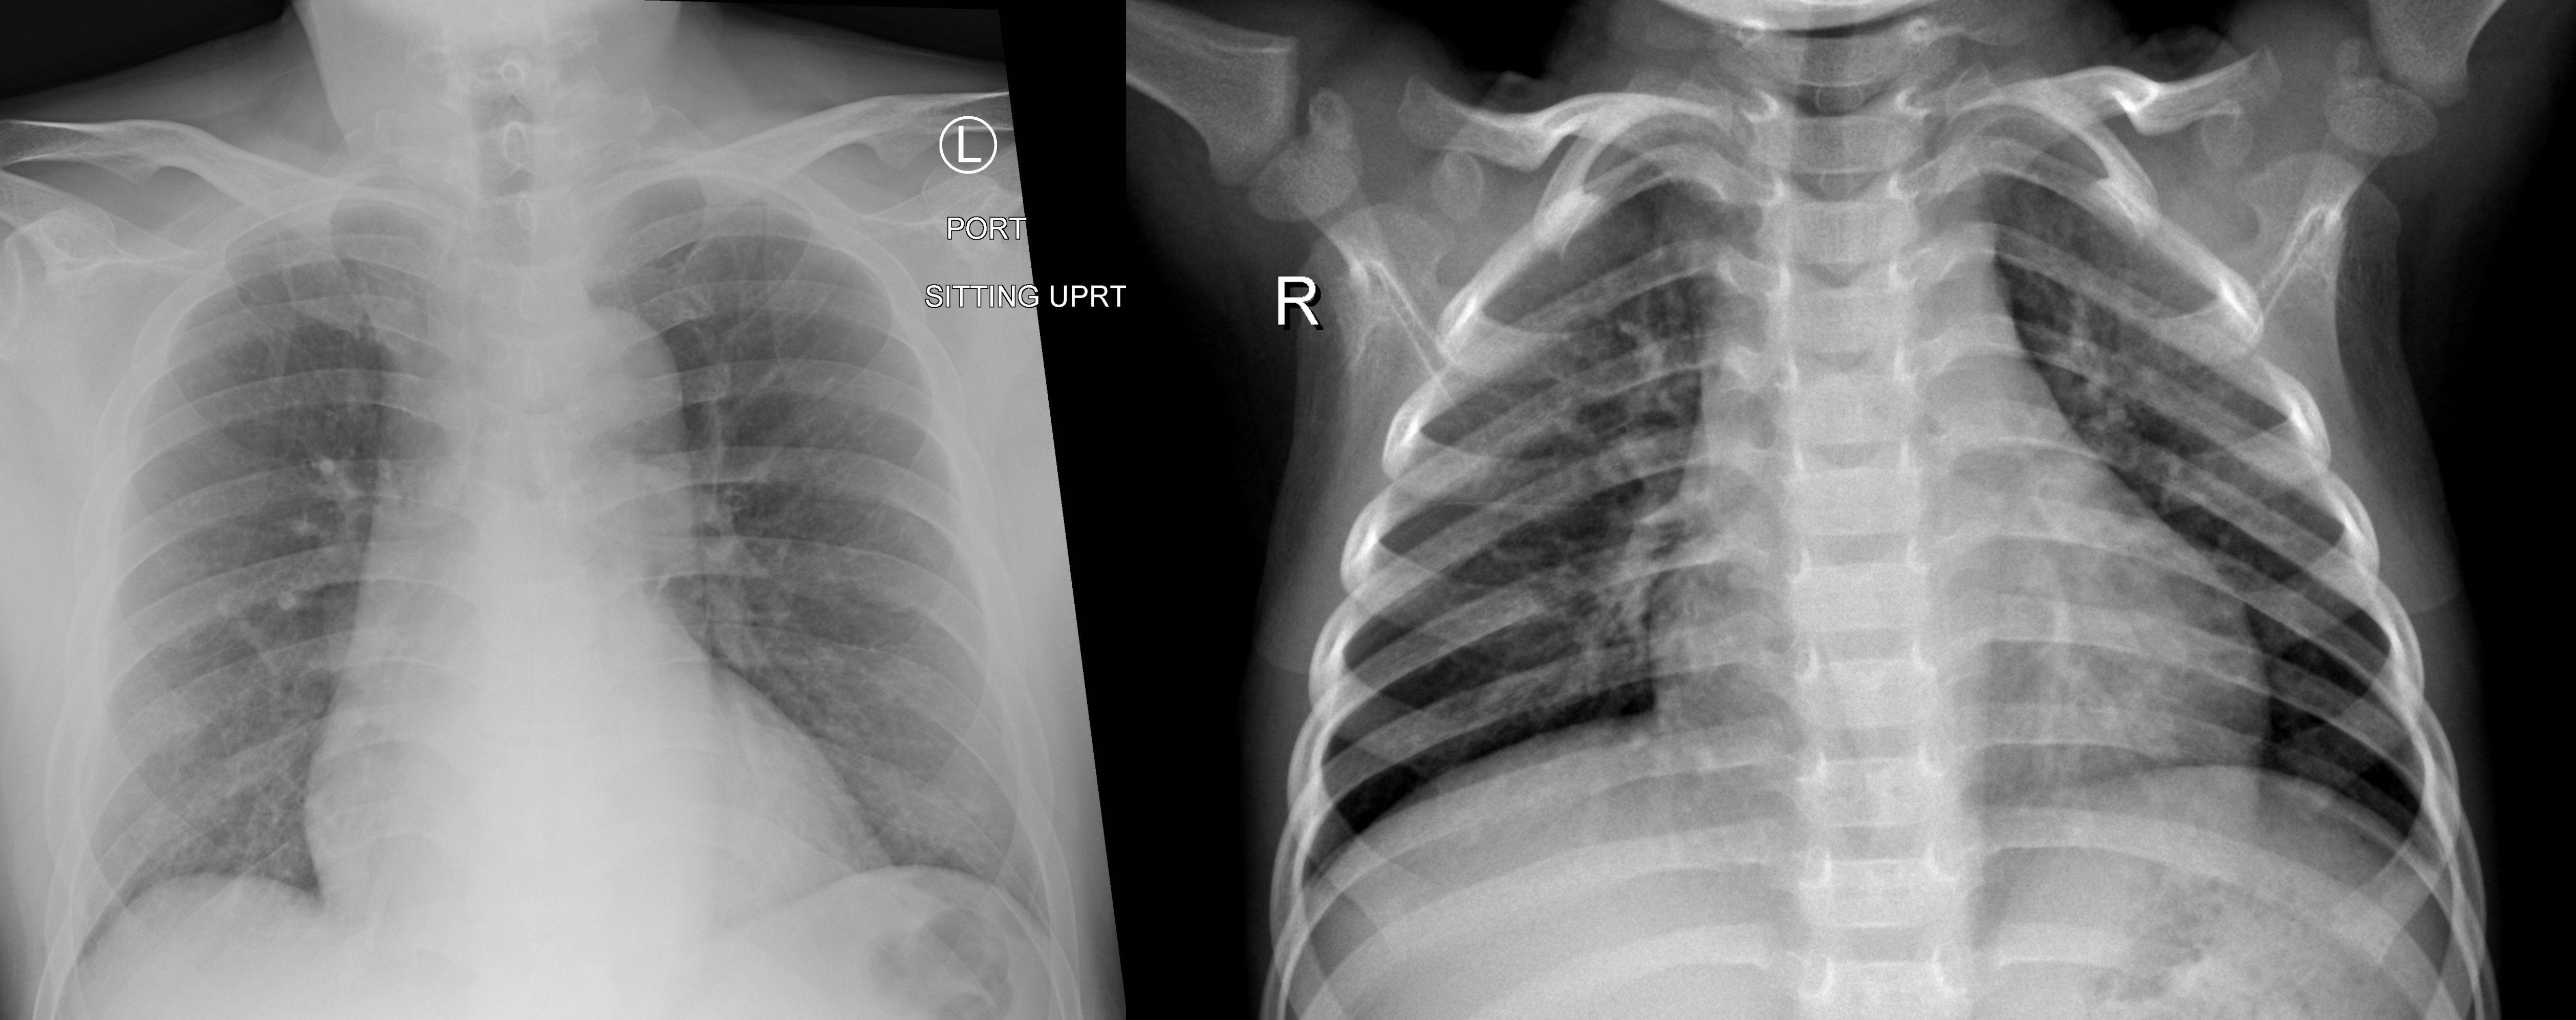
\includegraphics[width=16cm]{CNN_Data.jpg}
    \caption{COVID-19 and Normal Chest X-ray Images}
    \label{fig:def}
\end{figure}
\\In order to create the CNN model, Google Colaboratory, or Colab, is used in which Python codes can be written and executed on the browser. The benefits of Colab are no configuration required, free access to GPUs and the file can be easily shared with others. Image datasets can be easily uploaded into Google Colab with a few lines of code which is executed on the power of Google hardware (including GPUs and TPUs), regardless of the power of your machine. Google Colab is widely used for getting started on TensorFlow and making neural network models. 
\\The dataset is converted into a zip file to take up less space and is then uploaded onto Dropbox. The Dropbox link is shared on Google Colab, which quickly downloads the zip file. We unzip the file, and the dataset has successfully been uploaded into Google Colab. In order to build the model, Numpy, matplotlib, Keras in-built libraries are used. TensorFlow is running in the backend. 
\\The CNN model consists of two types of layers: Convolutional layers and Fully Connected Layers. A nine layered CNN model is created, consisting of three sets of stacked convolutional and pooling layers followed by two fully connected layers for classifying COVID-19 and normal x-ray images. There are four convolutional layers with filter sizes of 3 x 3 but having increasing filter numbers (32, 64,64,128) over the layers. 
%(MODEL IMAGE)
\begin{figure}[htp]
    \centering
    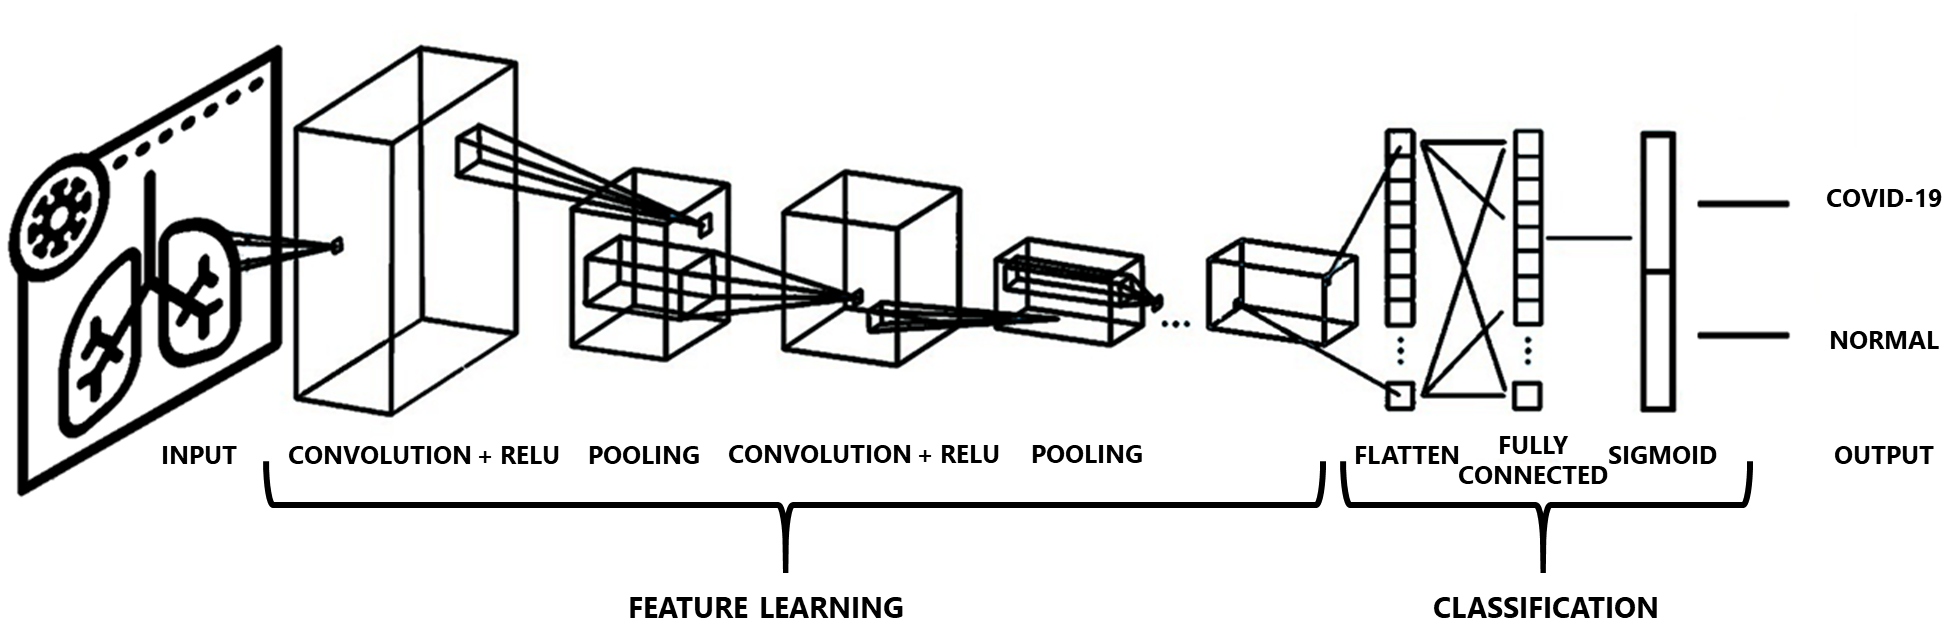
\includegraphics[width=16cm, height = 8cm]{CNN_Arch.png}
    \caption{Architechture of the CNN Model}
    \label{fig:ghi}
\end{figure}
\\The initial layers are small in the beginning because the lower layers detect features in small parts of the images and can find small patterns in the image as we go deeper into the layers, the receptive field of the CNN layer increases. The kernel size is 3 x 3, which is a standard choice. Activation of Relu layer is used in the convolutional layers for non-linearity. Since this is the first layer, we specify the input size as 224 x 224 x 3. There are three pooling layers with filter size 2 x 2 each which is the default size, by using Max Pooling, the receptive field of the layer increases.
\\The first convolutional layer is reshaped into 224 x 224 with three channels because the x-rays are RGB images. On carefully noticing the images, it is observed that the chest x-rays are not greyscaled images but RGB in nature because some pictures have a tone of blue or yellow. In the first set of a stacked convolutional layer, two convolutional layers of 3 x 3 kernel size have been used instead of one convolutional layer of 5 x 5 kernel size. Using two layers is advantageous to the model as it increases non-linearity in the model, and there are fewer parameters which in-turn reduce overfitting. The model can detect a higher level of features in images with the model layers deepening. After every pooling layer, a dropout layer is added to reduce the risk of overfitting with the dropout rate of 25\%.
\\After inputting the convolutional and pooling layers, the output shape has to be changed in order to go forward with the fully connected layers. Hence, the model is converted from a two-dimensional layer to one dimension by using a flattening layer and then connected to a fully connected layer. The fully connected layer uses the ReLu function for activation. For the output layer, there is only one filter applied since we have to classify the images between COVID-19 and Normal chest x-ray images. Due to this reason, the activation function of Sigmoid is used. 
\\The model is compiled with binary entropy loss and adam optimiser, which is the default optimiser function using accuracy metrics. This model uses 56 lakh parameters in total, which is trained from scratch. The input shape at the beginning is 224 x 224, which converts into 222 x 222 after the first convolutional layer. The shape is changed to 26 x 26 or 26 x 128 before the flattening layer. 
\\The in-built Keras Image Generator library is used to train the dataset. In order to aid data convergence, the dataset is rescaled for normalisation of RGB images by 1/255. Moreover, usage of sheer and zoom augmentation is inculcated, allowing the model to take random crops from images and zooming into the images with 20\% magnitude of the image.  Vertical flipping of the image has been restricted in order to get accurate results. For the validation dataset, the Image Generator library is used to rescale the images for normalisation by 1/255. 
\\For the training dataset, the flow from directory function is applied to reshape the image with a target size of 224 x 224, having a batch size of 32 and using binary classification to distinguish between COVID-19 and Normal Chest x-rays. The same has been done for the validation dataset. The input size of 224 x 224 is a standard choice used by data scientists. Most of the ImageNet problems are solved using this input size. The model would be difficult to train if the input size would be big, and it would be challenging to capture fine-grained features if the input size would be small. In the training process, 10 epochs are used with 8 steps per epoch.  
\\This model is simpler than other models like VGG16, ImageNet and TransferNet as it uses few parameters. The other models will not give good results since they contain over a million parameters. Since the dataset contains chest x-rays, the models would have to be carefully fine-tuned with several modifications which   Moreover, the dataset is too small and would hence lead to overfitting. The other models require at least 3000 images for training in order to give a good accuracy score.

\pagebreak
\section{Model Accuracy and Loss over Epochs}
\begin{figure}[htp]
    \centering
    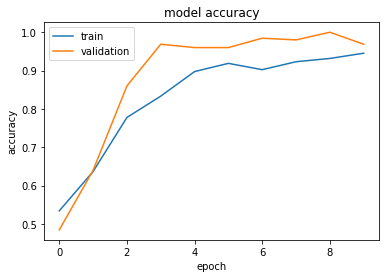
\includegraphics[width=9cm]{Model_Acc.png}
    \caption{Confusion Matrixr}
    \label{fig:abc}
\end{figure}

\begin{figure}[htp]
    \centering
    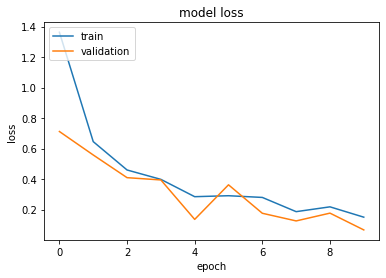
\includegraphics[width=9cm]{Model_Loss.png}
    \caption{Confusion Matrixr}
    \label{fig:abc}
\end{figure}

\pagebreak
\section{Results Obtained}
In order to get a summary of the results on a classification problem, a confusion matrix is computed to visually understand the results of the model. It summarises the correct and incorrect predictions broken down by each class. It shows how the classification model gets confused when it makes predictions and gives an insight not only into the magnitude of errors being made but also regarding the type of errors being made. 
$$\begin{array}{|l|l|l|}
\hline & \text { COVID-19 } & \text { NORMAL } \\
\hline \text { COVID-19 } & \text { True Positive } & \text { False Negative } \\
\hline \text { NORMAL } & \text { False Positive } & \text { True Negative } \\
\hline
\end{array}$$
\\Where,
\\True Positive: Observation is positive, the prediction is positive.
$$T P_{i}=\sum_{i=1}^{n} x_{i i}$$
\\False Negative: Observation is positive, the prediction is negative.
$$F N_{i}=\sum_{j=1} x_{i j}, j \neq i$$
\\False Positive: Observation is negative, the prediction is positive.
$$F P_{i}=\sum_{j=1}^{c} x_{j i}, j \neq i$$
\\True Negative: Observation is negative, the prediction is negative.
$$T N_{i}=\sum_{j=1}^{c} \sum_{k=1}^{c} x_{j k}, j \neq i, k \neq i$$
\\The Accuracy, Misclassification Error, Sensitivity Specificity and Precision of the model are evaluated from the Confusion Matrix to get a deeper understanding about model fitting.
\\\textbf{Accuracy: }Accuracy is used to measure the magnitude of the correctly predicted classes. It calculates how many COVID-19 and Normal patients have been correctly classified respectively. The formula is given as:
\begin{equation}\text{Precision}=\frac{T P+T N}{n}\end{equation}
\\\textbf{Misclassification Error: }Misclassification error is used to measure the magnitude of the wrongly predicted classes. It calculates the amount of COVID-19 and Normal patients who have been wrongly classified respectively. The formula is given as:
\begin{equation}\text{Misclassification Error} = 1 - Accuracy\end{equation}
\\\textbf{Sensivity: } Sensitivity is used to measure how the model is detecting the positive class. It calculates how many COVID-19 patients are correctly predicted. The formula is given as:
\begin{equation}\text {Sensitivity}=\frac{T P}{T P+F N}\end{equation}
\\\textbf{Specificity: } Specificity is used to measure how the model is detecting the negative class. It calculates how many Normal patients are correctly predicted. The formula is given as:
\begin{equation}\text {Specificity}=\frac{T N}{F P+T N}\end{equation}
\\\textbf{Precision:} Precision is used to measure the ability of the model in detection of only the relevant datapoints. It calculates the total number of positives present in the data. The formula is given as:
\begin{equation}\text{Precison}=\frac{ TP}{T P+F P}\end{equation}
\\The confusion matrix has been performed on the Validation dataset. The results of the confusion matrix are as follows:
%IMAGE OF CN
\begin{figure}[htp]
    \centering
    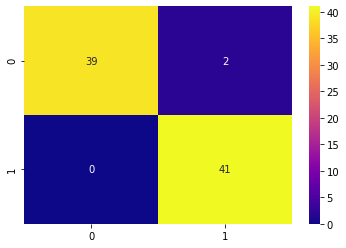
\includegraphics[width=7cm]{ConfusionMatrix.png}
    \caption{Confusion Matrixr}
    \label{fig:abc}
\end{figure}
%PROBLEM IN FORMATTING
\\On decoding the Confusion matrix, it is observed that out of 41 COVID-19 affected patients, there are 2 patients wrongly classified and, out of 41 Normal patients, 0 patients have been wrongly classified. In our model, 2 of the patients have been wrongly classified in total. 
$$\begin{array}{|c|c|c|c|c|}
\hline \text { Accuracy } & \text { Misclassification Error } & \text { Sensitivity } & \text { Specificity } & \text { Precision } \\
\hline 0.9756 & 0.0243 & 0.9512 & 1.000 & 1.000 \\
\hline
\end{array}$$
\\On evaluating the model, it is observed that the validation accuracy is 97\%. Although, it is a good accuracy score, there may be some cons to deploy this model since there could be some major consequences. For example, with a 97\% accuracy, the model would be able to rightly detect 97 patients out of 100 but would wrongly guess 3 patients. There can be a scenario where a patient can be misclassified, that is, a patient can be COVID-19 negative but the model states that he is COVID-19 positive. Hence, he will made to quarantined with patients who are COVID-19 positive leading to him getting affected. On the other hand, it may also happen that a patient can be COVID-19 positive but the model states that he is COVID-19 negative. This could be dangerous as he could spread the virus to other people in his surroundings. Thus, when it comes to medical imaging, one must be super cautious and must ought to have a good accuracy score as it is a question of human life. 

\pagebreak
\section{Conclusion}
Early prediction of COVID-19 patients is vital to prevent the spread of the disease to other people. The virus is relatively new and no official vaccine has been originated yet. Hence, humanity ought to find different ways to prevent COVID-19 from spreading to their surroundings in order to get back to normalcy as soon as possible. 
\\Chest X-ray images play a vital role in the detection of COVID-19. In this study, a CNN Model was used to detect COVID-19 using Chest X-ray images obtained from COVID-19 patients and Normal patients. CNN enables learning highly representative and hierarchical local image features directly from data. The model performance is 97\% which is a great accuracy score with the recent origins of the virus. Although this paper is only for educational and research purposes, not for medical purposes, it will aid doctors to make better decisions in clinical practice due to the higher performance of the model. 
\\However, the irregularities in annotated data remains the biggest challenge in coping with COVID-19 cases from Chest X-ray images. The limitations for this paper are:
\\a)	Lack of COVID-19 Chest X-rays due to the recent emergence of the virus. 
\\b)	No medical guidance was used for the analysis of the project. 
\\The future scope for this paper can be:
\\a)	To increase the dataset with more availability of data.
\\b)	To incorporate other infections like Viral Pneumonia and Bacterial Pneumonia.
\\c)	 To implement Gradient Class Activation Map (Grad-CAM) and Saliency maps in order to figure out the regions in which the infection has spread among the COVID Chest X-rays.
\\Nonetheless, the present work contributes to the possibility of a low-cost, rapid, and automatic diagnosis of COVID-19. Also, despite the fact that the appropriate treatment is not determined solely from an X-ray image, an initial screening of the cases would be useful, not in the type of treatment, but in the timely application of quarantine measures in the positive samples, until a more complete examination and a specific treatment or follow-up procedure is followed. An additional advantage of automatic detection of COVID-19 from medical imaging lies on the reduction of exposure of nursing and medical staff to the outbreak. 

\pagebreak
\section{References}
YZ

\end{document}